
% !TEX root = NotesDeCours.tex

\part{\bfseries Cinématique des écoulements}
\section{ Cinématique des écoulements}


\begin{frame}

  \color{bleu}

  \begin{flushleft}
    
    \Large
   	\bf
    
    Mécanique des fluides 

  \end{flushleft}
  
  \ligne{3} % remplace: \noindent \thickline{0.5mm}{150}

  \begin{flushright}

    \rm

    \textrm{David} \textsc{Fabre}
    
    \vspace{3mm}
    
    IMFT / UPS
    
    Département de Mécanique
    
%    brancher@imft.fr

  \end{flushright}


\begin{picture}(110, 30)(5, -22)
  \put( 5, -25){\includegraphics[height=50mm]{./Figures/gerris.jpg}}
  \put(68, -12){\color{gris} \slshape \small Dipôles tourbillonnaires générés }    	
  \put(68, -15){\color{gris} \slshape \small par une araignée d'eau (gerris)}
  \put(68, -18){\color{gris} \slshape \small se déplaçant à la surface de l'eau}
  \put(68, -23){\color{gris} \small \rm \copyright\ MIT}
\end{picture}

  \vspace{7mm}
  
  \begin{flushright}
    
    \Large
   	\bf
    
    3. Cinématique des fluides

  \end{flushright}

\end{frame}

%%%%%%%%%%%%%%%%%%%%%%%%%%%%%%%%%%%%%%%%%%%%%%%%%%%%%%%%%%%%%%%%%%%%%%%%%%%%%%%%%%%%%%%%%%%%%%%%%%%
%%%%%%%%%%%%%%%%%%%%%%%%%%%%%%%%%%%%%%%%%%%%%%%%%%%%%%%%%%%%%%%%%%%%%%%%%%%%%%%%%%%%%%%%%%%%%%%%%%%


%%%%%%%%%%%%%%%%%%%%%%%%%%%%%%%%%%%%%%%%%%%%%%%%%%%%%%%%%%%%%%%%%%%%%%%%%%%%%%%%%%%%%%%%%%
% Sommaire :
%%%%%%%%%%%%%%%%%%%%%%%%%%%%%%%%%%%%%%%%%%%%%%%%%%%%%%%%%%%%%%%%%%%%%%%%%%%%%%%%%%%%%%%%%%
\handout{
\begin{frame}{Sommaire}
\small  
\hspace*{2mm}
\begin{tabular}{cc}
		%&
  		\begin{minipage}{62mm}
  			\tableofcontents[]
      \vspace{15mm}
  		\end{minipage}
  		&   
  		\begin{minipage}{60cm}
		  \vspace*{-5mm}  
  			%\includegraphics[width=40mm]{vagues.jpg} 
  		\end{minipage}
  	\end{tabular}
\vspace{0mm}
\end{frame}
}



%==================================================================================================
\subsection{Description du mouvement d'un fluide}
%==================================================================================================

\subsubsection{Formalismes lagrangien et eulérien}

%--------------------------------------------------------------------------------------------------
\begin{frame}{Description lagrangienne : définition}
%--------------------------------------------------------------------------------------------------

\small

\begin{center}
	\begin{picture}(110, 40)(0, 3)
		  \put(63, 5){\includegraphics[width=40mm]{lagrangien.png}}
		  \put(65, 15){\colorbox{white}{$\myvec{X}(t, \myvec{X}_0)$}}
		  \put(80, 30){$F(t, \myvec{X}_0)$}
		  \put(74, 44){$\myvec{X}_0$}
		  \put(76.5, 34){$t$}
		  \put(93, 24){\color{red} trajectoire}
		\put(0, 25){%

\begin{minipage}{60mm}

\medskip


				\mybaselineskip{1.2}{

				La {\bf description Lagrangienne} consiste à décrire l'écoulement d'un fluide par la donnée,				
				\smallskip
				à chaque instant $t$, et pour chaque \textcolor{vert}{\em particule fluide} (indexée par la position $\myvec{X}_0$ qu'elle occupait à l'instant  $t=0$) :
\pause
\small
				\medskip
				\begin{itemize}
				\item
					de la \textcolor{vert}{trajectoire} $\myvec{X}(t ; \myvec{X}_0)$, 
					\\
\pause
				\item
					de l'évolution des grandeurs physiques $F(t ; \myvec{X}_0)$ 
					\textcolor{vert}{attachées à la particule fluide}
					(et donc transportées par elle)
					
					\smallskip
					Ici $F(t ; \myvec{X}_0)$ peut désigner la masse volumique $\rho$, 					l'énergie interne $e$ ou encore la température $T$ de la particule $\myvec{X}_0$.
	
				\end{itemize}
}
			\end{minipage}}
	\end{picture}
\end{center}

%\pause

%\begin{center}
%\textcolor{rouge}{"On suit la matière dans son mouvement"}
%\end{center}


\pause
\medskip

{\bf Remarques:}

\begin{itemize}
\item
Dans ce formalisme, $\myvec{X}_0$ est à considérer comme un 'label', pas comme une variable ; $\myvec{X}(t ; \myvec{X}_0)$ et $F(t ; \myvec{X}_0)$ sont des fonctions d'une seule variable $t$. 

On peut donc utiliser la notation $d/dt = \dot{()}$ 

\pause 
\item 
{\color{bleu} \tiny

\slshape
La vitesse de la particule fluide est donc donnée par 
$\dot{\myvec{X}}(t; \myvec{X}_0) \equiv \ddt{}\myvec{X}(t; \myvec{X}_0)$

%\smallskip

\hspace{24mm} et son accélération par 
$\displaystyle \ddot{\myvec{X}}(t; \myvec{X}_0) \equiv \frac{ d^2 }{d t^2}\myvec{X}(t; \myvec{X}_0)$
}


\pause
\item Le formalisme repose sur le concept de "Particule fluide", définie comme un {\em point matériel supposé se déplacer à la "vitesse du fluide". }

Concept faussement intuitif !

\end{itemize}

\vspace{0mm}

\end{frame}

%--------------------------------------------------------------------------------------------------
\begin{frame}{Description lagrangienne : exemple}
%--------------------------------------------------------------------------------------------------

\small

\begin{center}
	\begin{picture}(110, 75)(1, -2)
		\put(0, 0){\includegraphics[width=25mm]{bouee_derivante.png}}
		\put(0, 52){\includegraphics[width=25mm]{photo_bouee.png}}
		\put(28, 63){%
			\begin{minipage}{80mm}
				Bouée dérivante : 
				\\
				\hspace*{10mm} mesure de la température de surface de la mer,
				\\
				\hspace*{10mm} de la pression atmosphérique et des courants de surface. 
				
				\pause
				\medskip
				
				Principe : en dérivant avec le courant, la bouée suit toujours les mêmes particules fluides 		
				(celles qui l'entourent) $\rightarrow$ \textcolor{rouge}{description lagrangienne}

%				\medskip
%				
%				Les mesures de température de la mer effectuées par les bouées dérivantes sont très utiles 
%				pour étalonner les mesures effectuées par satellite. 
%				Elles permettent notamment de corriger l'atténuation du signal due à l'atmosphère 
%				et à valider les modèles d'analyse et de prévision de la circulation océanique 
%				basés sur des observations satellitaires (altimétrie).
  
			\end{minipage}}
		\put(28, 0){\includegraphics[height=49.27mm]{southatlantic.png}}
		\put(85, 22){%
			\begin{minipage}{35mm}
				La trajectoire des bouées \\
				est suivie par le système \\
				de positionnement Argos. 
	 		\end{minipage}}
		\put(89, 15){\vector(-1, 0){5}}
		\put(89, 15){\line(0, 1){2}}
	\end{picture}
\end{center}

    

\vspace{0mm}

\end{frame}


%--------------------------------------------------------------------------------------------------
\begin{frame}{Description eulérienne : définition}
%--------------------------------------------------------------------------------------------------

\small

\begin{center}
	\begin{picture}(110, 35)(0, 0)
		  \put(67, 0){\includegraphics[width=40mm]{eulerien.pdf}}
		  \put(75, 4){\colorbox{white}{$\myvec{x}$}}
		  \put(90.5, 10.7){\setlength{\fboxsep}{0.5mm}\colorbox{white}{$f(\myvec{x}, t)$}}
		  \put(98, 7.7){\setlength{\fboxsep}{0.5mm}\colorbox{white}{$\myvec{u}(\myvec{x}, t)$}}
		  \put(83.5, 16){\colorbox{white}{\color{blue} \tiny point}}
		  \put(81.5, 13.5){\setlength{\fboxsep}{0.5mm}\colorbox{white}{\color{blue} \tiny géométrique}}
		\put(0, 20){%
			\begin{minipage}{62mm}

				%\vspace{-32mm}

				\mybaselineskip{1.2}{
La {\bf description Eulérienne } d'un écoulement consiste à décrire celui-ci par la donnée, à chaque instant $t$ et en tout \textcolor{vert}{point géométrique}  $\myvec{x}$ de l'espace :
				\medskip \pause

				\begin{itemize}
				\item
			du \textcolor{vert}{champ (vectoriel) de vitesse $\myvec{u}(\myvec{x}, t)$}, 
										\pause
				\item
			des \textcolor{vert}{champs scalaires}  $f(\myvec{x}, t)$
			où $f(\myvec{x}, t)$ peut désigner la masse volumique $\rho$, l'énergie interne $e$ 
			ou la température $T$.		\end{itemize}
}
			\end{minipage}}
	\end{picture}
\end{center}

\smallskip \pause

%\mybaselineskip{1.2}{
%Les quantités $\myvec{u}(\myvec{x}, t)$ et $f(\myvec{x}, t)$ définissent des champs, 
%dits eulériens, respectivement de vitesse et, par exemple, de masse volumique 
%$\rho(\myvec{x}, t)$, de concentration $n_i(\myvec{x}, t)$ ou de température $T(\myvec{x}, t)$.
%}

\bigskip 
\pause
{\bf Remarque :}

Sous l'hypothèse des milieux continus, on a vu qu'on peut définir rigoureusement les champs 
$\myvec{u}(\myvec{x}, t)$, $\rho(\myvec{x}, t)$ et  $T(\myvec{x}, t)$ par moyennage sur un $VER$ défini au voisinage de chaque point $\vec x$. 

\color{bleu}{(cf. chap. 2).} 

\medskip 

La définition eulérienne est donc finalement plus rigoureuse que la définition lagrangienne !
\vspace{0mm}

\end{frame}






%--------------------------------------------------------------------------------------------------
\begin{frame}{Description eulérienne : exemple}
%--------------------------------------------------------------------------------------------------

\small

\begin{center}
	\begin{picture}(125, 50)(5, 0)
		\put(5, 30){%
			\begin{minipage}{55mm}
				\textbf{Anémomètre fixe \\ avec mesure de la qualité de l'air}
				
				\medskip
				
				on mesure la vitesse et la concentration \\ en polluants de particules fluides
				différentes \\ au cours du temps : 
				
				\medskip
				
				{\slshape on ne suit pas la matière dans son mouvement}
				
				\medskip
				
				$\rightarrow$ \textcolor{rouge}{description eulérienne}
							\end{minipage}}
		\put(65, 0){\includegraphics[width=40mm]{anemometre.jpg}}
	\end{picture}
\end{center}


\vspace{0mm}

\end{frame}

%--------------------------------------------------------------------------------------------------
\begin{frame}{Choix du formalisme}
%--------------------------------------------------------------------------------------------------

\small

\pause

\begin{itemize}
\item<2->
La description \textbf{lagrangienne} est en générale privilégiée en mécanique des solides, 
\\
principalement intéressée par les déformations et les déplacements courts ou faibles
\\
(pas d'écoulement $\Rightarrow$ les particules solides restent dans le domaine d'étude)

\medskip

\item<3->
Au contraire la mécanique des fluides s'intéresse aux fluides en écoulement 
\\
(taux de déformations et taux de déplacement = vitesse des particules fluides) : 
\\
les particules fluides sont susceptibles de traverser le domaine d'étude pour en sortir.
\end{itemize}

\begin{overprint}

  \onslide<2>   
  
  \begin{center}
		\begin{picture}(50, 20)(0, 0)
			\put(0, 0){\includegraphics[width=50mm]{deformation_balle.png}}
		\end{picture}
	\end{center}

  \onslide<3>   
  
  \begin{center}
		\begin{picture}(50, 25)(0, 0)
			\put(0, 0){\includegraphics[width=50mm]{streamlines_car.jpg}}
		\end{picture}
	\end{center}

  \onslide<4>   
  
  \begin{center}
		\begin{picture}(50, 25)(0, 0)
			\put(0, 0){\includegraphics[width=50mm]{streamlines_car.jpg}}
			\put(-0.1, 12.8){\color{white} $\bullet$}
			\put(-0.04, 12.98){\tiny \color{red} $\bullet$}
		\end{picture}
	\end{center}

  \onslide<5>   
  
  \begin{center}
		\begin{picture}(50, 25)(0, 0)
			\put(0, 0){\includegraphics[width=50mm]{streamlines_car.jpg}}
			\put(6., 13.2){\color{white} $\bullet$}
			\put(6.06, 13.38){\tiny \color{red} $\bullet$}
		\end{picture}
	\end{center}

 \onslide<6>   

  \begin{center}
		\begin{picture}(50, 25)(0, 0)
			\put(0, 0){\includegraphics[width=50mm]{streamlines_car.jpg}}
			\put(13.4, 14.0){\color{white} $\bullet$}
			\put(13.46, 14.18){\tiny \color{red} $\bullet$}
		\end{picture}
	\end{center}

  \onslide<7>   
  
  \begin{center}
		\begin{picture}(50, 25)(0, 0)
			\put(0, 0){\includegraphics[width=50mm]{streamlines_car.jpg}}
			\put(21.4, 14.9){\color{white} $\bullet$}
			\put(21.46, 15.08){\tiny \color{red} $\bullet$}
		\end{picture}
	\end{center}

  \onslide<8>   
  
  \begin{center}
		\begin{picture}(50, 25)(0, 0)
			\put(0, 0){\includegraphics[width=50mm]{streamlines_car.jpg}}
			\put(29.9, 15.5){\color{white} $\bullet$}
			\put(29.96, 15.68){\tiny \color{red} $\bullet$}
		\end{picture}
	\end{center}

  \onslide<9>   
  
  \begin{center}
		\begin{picture}(50, 25)(0, 0)
			\put(0, 0){\includegraphics[width=50mm]{streamlines_car.jpg}}
			\put(40.1, 14.95){\color{white} $\bullet$}
			\put(40.16, 15.13){\tiny \color{red} $\bullet$}
		\end{picture}
	\end{center}

  \onslide<10>   
  
  \begin{center}
		\begin{picture}(50, 25)(0, 0)
			\put(0, 0){\includegraphics[width=50mm]{streamlines_car.jpg}}
			\put(48.1, 14.25){\color{white} $\bullet$}
			\put(48.16, 14.43){\tiny \color{red} $\bullet$}
		\end{picture}
	\end{center}
	
  \onslide<11>   
  
  \begin{center}
		\begin{picture}(50, 25)(0, 0)
			\put(0, 0){\includegraphics[width=50mm]{streamlines_car.jpg}}
			\put(49.1, 14.15){\color{white} $\bullet$}
			\put(49.16, 14.33){\tiny \color{red} $\bullet$}
			\put(-0.1, 12.8){\color{white} $\bullet$}
			\put(-0.04, 12.98){\tiny \color{red} $\bullet$}
		  \put(-27, 20){\color{red}nouvelle particule fluide}
		  \put(52, 21){\color{red}particule fluide sortante}
		  \put(-5, 18.5){\color{red}\vector(1, -1){5}}
		  \put(55.5, 20.1){\color{red}\vector(-1, -1){5}}
		\end{picture}

	\bigskip

	Il est donc difficile de suivre la matière dans son mouvement, 
	\\
	et on privilégiera alors une description \textbf{eulérienne}.

	\end{center}

\end{overprint}


\vspace{10mm}

\end{frame}


%--------------------------------------------------------------------------------------------------
\subsubsection{Correspondance entre formalismes}
%--------------------------------------------------------------------------------------------------
\begin{frame}{Relations entre descriptions lagrangienne et eulérienne}
%--------------------------------------------------------------------------------------------------

\small


Si $\myvec{X}_0$ désigne la particule fluide située en $\myvec{x}$ à l'instant $t$
\[
	\color{rouge}
	\myvec{X}(t; \myvec{X}_0) = \myvec{x}
\]

\pause

alors, par définition :

{\color{rouge}
\begin{eqnarray}
	\myvec{u}(\myvec{x}, t) & = & \dot{\myvec{X}}\left ( t; \myvec{X}_0 \right )
	\quad \mbox{\color{black}(vitesse de la particule $\myvec{X}_0$)}
	\\ \pause
	f(\myvec{x}, t) & = & F\left ( t; \myvec{X}_0 \right )
	\quad \mbox{\color{black}(par ex., température de la particule $\myvec{X}_0$)}
\end{eqnarray}
}

\bigskip

$\rightarrow$ On peut ainsi passer d'une formulation à l'autre à l'aide de ces relations.

\medskip
%\hfill \textsl{\color{vert} cf. exercice du sablier en TD}

\vspace{20mm}

\end{frame}


%==================================================================================================
\subsection{Dérivée matérielle}
%==================================================================================================

%--------------------------------------------------------------------------------------------------
\subsubsection{Dérivée particulaire d'un champ scalaire}
%--------------------------------------------------------------------------------------------------
\iffalse
\begin{frame}{Champ scalaire : rappel mathématique}
%--------------------------------------------------------------------------------------------------

\small

En notant $\myvec{x} = (x, y, z)$ le vecteur position 
et $d\myvec{x} = (dx, dy, dz)$ le déplacement élémentaire,
alors tout champ scalaire $f(\myvec{x})$ accepte le développement limité suivant :

\begin{eqnarray*}
f(\myvec{x} + d\myvec{x}) & = & f(x+dx, y+dy, z+dz)
\\
& = & f(x, y, z) + {\color{rouge}\dpdx{f}(x, y, z)\,dx + \dpdy{f}(x, y, z)\, dy + \dpdz{f}(x, y, z)\, dz} + \ldots 
\end{eqnarray*}

Soit :
\[
	f(\myvec{x} + d\myvec{x}) \approx f(\myvec{x}) + {\color{rouge}\gradient f \cdot d\myvec{x}}
\]

\bigskip

\pause

Par extension on en déduit que pour tout champ $f(\myvec{x}, t)$ :
\[
	f(\myvec{x} + d\myvec{x}, {\color{rouge}t+dt}) \approx f(\myvec{x}, t) + \gradient f \cdot d\myvec{x}
	+ {\color{rouge} \dpdt{f}(\myvec{x}, t) \; dt} 
\]


\vspace{20mm}

\end{frame}
\fi

%--------------------------------------------------------------------------------------------------
\begin{frame}{Variation temporelle d'une quantité scalaire transportée par une particule fluide}
%--------------------------------------------------------------------------------------------------

\small
			

\begin{picture}(0, 40)(10, -5)
		\put(10, 15){
		\begin{minipage}{60mm}
			\mybaselineskip{1.2}{
			Soit $\myvec{X}_0$ la particule fluide
			située en $\myvec{x}$ à l'instant $t$ :
			\begin{center}
				$\myvec{X}(t; \myvec{X}_0) = \myvec{x}$
			\end{center}
			}			
\bigskip

Comment calculer la \textcolor{vert}{variation temporelle} de $F$ :

\begin{center}
$ \displaystyle
	\dot{F}(t; \myvec{X}_0) 
	= 
	\lim_{dt\rightarrow 0} \frac{F(t+dt; \myvec{X}_0) - F(t; \myvec{X}_0)}{dt}
$
			\end{center}

en fonction des champs eulériens $f(\myvec{x}, t)$ et $\myvec{u}(\myvec{x}, t)$ ?
		\end{minipage}
		}
		\put(78, -5){\includegraphics[width=35mm, height=40mm]{derivee_particulaire.png}}
		\put(83, 7){\footnotesize \colorbox{white}{$\myvec{x}$}}
		\put(86, 3){\footnotesize \colorbox{white}{$\myvec{x}+d\myvec{x}$}}
		\put(93, 13){\footnotesize $d\myvec{x}$}
		\put(90, 24){\footnotesize $\myvec{X}(t; \myvec{X}_0)$}
		\put(90, 21){\footnotesize $F(t; \myvec{X}_0) = f(\myvec{x}, t)$}
		\put(99, 15){\footnotesize $\myvec{X}(t+dt; \myvec{X}_0)$}
		\put(98, 6){\footnotesize \setlength{\fboxsep}{0.5mm} \colorbox{white}{$F(t+dt; \myvec{X}_0) =$}}
		\put(98, 3){\footnotesize \setlength{\fboxsep}{0.5mm}\colorbox{white}{$f(\myvec{x}+d\myvec{x}, t+dt)$}}
\end{picture}

			
\vspace{10mm} \pause

[Démonstration\ldots] \hfill $\longrightarrow$ \quad
$ \displaystyle \color{rouge}
\dot{F}(t, \myvec{X}_0) 
	= 
	\lim_{dt\rightarrow 0} \frac{F(t+dt; \myvec{X}_0) - F(t; \myvec{X}_0)}{dt}
	= 
	\dpdt{f} + \gradient f \cdot \myvec{u} 
	$
\vspace{10mm}

\end{frame}

%--------------------------------------------------------------------------------------------------
\begin{frame}{Dérivée particulaire d'un champ scalaire}
%--------------------------------------------------------------------------------------------------

\small

\textbf{Définition :} \medskip

On appelle \textcolor{vert}{dérivée particulaire} (ou dérivée matérielle) 
du champ eulérien $f(\myvec{x}, t)$ la quantité

\[
	\color{rouge}
	\ddt{f} 
	=
	\underbrace{\dpdt{f}}_{\mbox{ dérivée intrinsèque}} +  \underbrace{\gradient f \cdot \myvec{u}}
	_{\mbox{ dérivée convective}}

\]

\medskip

Remarque : la dérivée particulaire est parfois aussi notée $\dfrac{Df}{Dt}$.

\bigskip
\pause

\textbf{Interprétation physique :} \medskip

Cette dérivée s'interprète comme le taux de variation temporelle de la grandeur physique associée au champ $f$ lorsque l'on suit dans son mouvement la particule fluide transportant cette quantité 
passant en $\myvec{x}$ à l'instant $t$ :

\[
	{\color{rouge}
	\ddt{f}(\myvec{x},t) = \dot{F}(t; \myvec{X}_0)}
	\quad \mbox{avec $\myvec{X}(t; \myvec{X}_0) = \myvec{x}$} 
\]

\pause

\textbf{Exemple  :} 

\medskip
{\tiny 
Par une belle journée d'été une Montgolfière s'élève dans le ciel. Le pilote observe sur son thermomètre une baisse de température. Celle-ci est-elle de nature intrinsèque ou convective ?

\smallskip

Le soir, en pliant sa toile, le pilote observe de nouveau une baisse de température.  Intrinsèque ou convective ?
}


\vspace{20mm}

\end{frame}
\comment{
%--------------------------------------------------------------------------------------------------

%--------------------------------------------------------------------------------------------------
\begin{frame}{Champ vectoriel : rappel mathématique}
%--------------------------------------------------------------------------------------------------

\small

En notant $\myvec{x} = (x, y, z)$ le vecteur position 
et $d\myvec{x} = (dx, dy, dz)$ le déplacement élémentaire,
alors tout champ vectoriel $\myvec{f}$ accepte le développement limité suivant :

\begin{eqnarray*}
\myvec{f}(\myvec{x} + d\myvec{x}) & = & \myvec{f}(x+dx, y+dy, z+dz)
\\
& = & \myvec{f}(x, y, z) + \dpdx{\myvec{f}}(x, y, z)\,dx + \dpdy{\myvec{f}}(x, y, z)\, dy + \dpdz{\myvec{f}}(x, y, z)\, dz + \ldots
\\
& = & \myvec{f}(x, y, z) 
      + \left ( {\color{rouge} dx\,\dpdx{} + dy\,\dpdy{} + dz\,\dpdz{}} \right ) \myvec{f} + \ldots
\end{eqnarray*}

D'où :
\begin{eqnarray*}
	\myvec{f}(\myvec{x} + d\myvec{x}) 
	& \approx &
	\myvec{f}(\myvec{x}) + \left ( {\color{rouge} d\myvec{x} \cdot \gradient} \right ) \myvec{f}  
	\\
	& \approx & 
	\myvec{f}(\myvec{x}) + \color{rouge}  {\ggradient \left ( \myvec{f} \, \right ) \cdot d\myvec{x}} 
\end{eqnarray*}

\bigskip



\medskip

Par extension on en déduit que pour tout champ vectoriel $\myvec{f}(\myvec{x}, t)$ :
\begin{eqnarray*}
	\myvec{f}(\myvec{x} + d\myvec{x}, {\color{rouge}t+dt}) 
	& \approx & 
	\myvec{f}(\myvec{x}, t) + 
	\left ( d\myvec{x} \cdot \gradient \right ) \myvec{f}
	+ {\color{rouge} \dpdt{\myvec{f}}(\myvec{x}, t) \; dt} 
	\\
	& \approx &
	\myvec{f}(\myvec{x}, t) + 
	\ggradient \left ( \myvec{f} \, \right ) \cdot d\myvec{x}
	+ {\color{rouge} \dpdt{\myvec{f}}(\myvec{x}, t) \; dt} 
\end{eqnarray*}

Rappel de MMC : le gradient d'un vecteur est un tenseur défini par la notation indicielle 
$$
{\left( \ggradient \myvec{f} \, \right ) }_{ij} = \left( \partial f_i/\partial x_j \right) 
$$


\vspace{0mm}

\end{frame}
}

%\subsubsection{Accélération d'une particule fluide}

\subsubsection{Accélération d'une particule fluide}

%--------------------------------------------------------------------------------------------------
\begin{frame}{Accélération d'une particule fluide}
%--------------------------------------------------------------------------------------------------

\small

\begin{picture}(0, 40)(10, -5)
		\put(10, 15){
		\begin{minipage}{60mm}
			\mybaselineskip{1.2}{
			Soit $\myvec{X}_0$ la particule fluide
			située en $\myvec{x}$ à l'instant $t$ :
			\begin{center}
				$\myvec{X}(t; \myvec{X}_0) = \myvec{x}$
			\end{center}
		}		
\bigskip

Comment calculer l'\textcolor{vert}{accélération} cette particule fluide :

\begin{center}
$ \displaystyle
	\myvec{a}(t, \myvec{X}_0) 
	= 
	\lim_{dt\rightarrow 0} \frac{\dot{\myvec{X}}(t+dt; \myvec{X}_0) - \dot{\myvec{X}}(t; \myvec{X}_0)}{dt}
$
			\end{center}

en fonction du champ eulérien de vitesse $\myvec{u}(\myvec{x}, t)$ ?
		\end{minipage}
		}
		\put(78, -5){\includegraphics[width=35mm, height=40mm]{derivee_particulaire.png}}
		\put(83, 7){\footnotesize \colorbox{white}{$\myvec{x}$}}
		\put(86, 3){\footnotesize \colorbox{white}{$\myvec{x}+d\myvec{x}$}}
		\put(93, 13){\footnotesize $d\myvec{x}$}
		\put(90, 24){\footnotesize $\myvec{X}(t; \myvec{X}_0)$}
		\put(90, 21){\footnotesize $F(t; \myvec{X}_0) = f(\myvec{x}, t)$}
		\put(99, 15){\footnotesize $\myvec{X}(t+dt; \myvec{X}_0)$}
		\put(98, 6){\footnotesize \setlength{\fboxsep}{0.5mm} \colorbox{white}{$F(t+dt; \myvec{X}_0) =$}}
		\put(98, 3){\footnotesize \setlength{\fboxsep}{0.5mm}\colorbox{white}{$f(\myvec{x}+d\myvec{x}, t+dt)$}}
\end{picture}

			
\vspace{5mm} \pause

[Démonstration\ldots] \hfill $\longrightarrow$ \quad
$ \displaystyle \color{rouge}
	\myvec{a}(t, \myvec{X}_0) 
	=
	\lim_{dt\rightarrow 0} 
	\frac{\dot{\myvec{X}}(t+dt; \myvec{X}_0) - \dot{\myvec{X}}(t; \myvec{X}_0)}{dt}	=	
	 \dpdt{\myvec{u}}
	%+\left ( \myvec{u} \cdot \gradient \right ) \myvec{u} 
	+{\ggradient \left ( \myvec{u} \, \right ) \cdot \myvec{u}} 
	$

\pause
\medskip



\textbf{Remarque  :}  autre notation possible  \medskip

%En introduisant la dérivée particulaire du champ de vitesse eulérien $\myvec{u}(\myvec{x}, t)$
\[
	\myvec{a}  
	=  \dpdt{\myvec{u}} + \left ( \myvec{u} \cdot \gradient \right )\myvec{u} 
\]
%cette quantité s'interprète comme l'\textcolor{vert}{accélération de la particule fluide 
%qui passe en $\myvec{x}$ à l'instant $t$}.
$\left ( \myvec{u} \cdot \gradient \right )\myvec{u}$ : Notation "pré-MMC" a interpréter "composante par composante", mais qui ne marche qu'en coordonnées cartésiennes !

(cf. formulaire, annexe D pour l'expression de ${\ggradient \left ( \myvec{u})}$ et de l'accélération en coordonnés cylindriques et sphériques).


\vspace{3mm}

\end{frame}

%--------------------------------------------------------------------------------------------------
\begin{frame}{Généralisation : dérivée particulaire d'un champ vectoriel}
%--------------------------------------------------------------------------------------------------

\small

\textbf{Définition :} \medskip

On appelle \textcolor{vert}{dérivée particulaire} (ou dérivée matérielle) 
du champ eulérien vectoriel $\myvec{f}(\myvec{x}, t)$ la quantité

\[
	\color{rouge}
	\ddt{\myvec{f}} 
		=
	\dpdt{\myvec{f}} + \ggradient \left ( \myvec{f} \, \right ) \cdot \myvec{u} 
	=
	\dpdt{\myvec{f}} + \left( \myvec{u} \cdot \gradient \right ) \myvec{f} 

\]


\bigskip

\textbf{Interprétation physique :} \medskip

Cette dérivée s'interprète comme le taux de variation temporelle de la grandeur physique associée au champ vectoriel $\myvec{f}$ lorsque l'on suit dans son mouvement la particule fluide transportant cette quantité passant en $\myvec{x}$ à l'instant $t$ :

\[
	{\color{rouge}
	\ddt{\myvec{f}}(\myvec{x},t) = \dot{\myvec{F}}(t, \myvec{X}_0)}
	\quad \mbox{où $\myvec{X}(t, \myvec{X}_0) = \myvec{x}$} 
\]

\textbf{Exemples :} \medskip

$\myvec{F}(t, \myvec{X}_0)$ peut représenter la vitesse de la particule fluide, 
sa quantité de mouvement ou son vecteur rotation instantanée.

\vspace{10mm}

\end{frame}




\subsubsection{Dérivée matérielle d'une quantité intégrale}

%%--------------------------------------------------------------------------------------------------
%\begin{frame}{Visualisation}
%%--------------------------------------------------------------------------------------------------
%
%\small
%
%Les écoulements peuvent être visualisés par le tracé des certaines courbes représentatives
%et descriptives : trajectoires, lignes de courant et lignes d'émission.
%
%\vspace{50mm}
%
%\end{frame}
%


%==================================================================================================
%\subsubsection{Flux d'une quantité à travers une surface}
%==================================================================================================
%--------------------------------------------------------------------------------------------------
\begin{frame}{Flux d'une quantité à travers une surface (rappel)}
%--------------------------------------------------------------------------------------------------

\small

Soit une quantité scalaire $f$  transportée par un écoulement de vitesse $\vec{u}$.
\smallskip

\begin{itemize}

\item En considérant une surface $\cal S$ séparant deux domaines $(1)$ et $(2)$,

\smallskip

\item[] on définit le {\em Flux} de $f$ à travers la surface (orientée de 1 vers 2):

$$
\Phi_{f,  ({\cal S}, 1 \rightarrow 2)} = \int_{\cal S} f \vec{u} \cdot  \vec {n}_{1\rightarrow 2} \, dS
$$

{\color{vert} Démonstration (...)} 

\pause 
\medskip

\pause
\medskip
\item Exemple : flux volumique ($f=1$) :
$$
\Phi_1 =  \int_{\cal S} \vec{u} \cdot  \vec {n}_{1\rightarrow 2} \, dS
$$

\item Pour une surface fermée de normale {\em sortante} $\vec{n}$, on définit le flux {\em sortant} :
$$
\Phi_{f} = \oint_{\cal S} f \vec{u} \cdot  \vec {n} \, dS
$$




\pause
\bigskip

\item {\bf Généralisation : } pour une quantité vectorielle $\vec{f}$ :
 
$$
\vec{\Phi}_{\vec{f},  ({\cal S}, 1 \rightarrow 2)} = \int_{\cal S} \vec{f} \left( \vec{u} \cdot  \vec {n}_{1\rightarrow 2} \right) \, dS
= \int_{\cal S} \left( \vec{f} \otimes \vec{u} \right) \cdot  \vec {n}_{1\rightarrow 2} \, dS
$$


\pause
\medskip
\item De même pour une surface fermée , on définit le flux {\em sortant} :
$$
\vec{\Phi}_{\vec{f}} = \oint_{\cal S} \vec{f} \left( \vec{u} \cdot  \vec {n} \right)\, dS
= \oint_{\cal S} \left( \vec{f} \otimes \vec{u} \right) \cdot  \vec {n} \, dS
$$

\end{itemize}
\end{frame}



%--------------------------------------------------------------------------------------------------
\begin{frame}{Théorème du transport}
%--------------------------------------------------------------------------------------------------

\small

Considérons un {\em domaine matériel } mobile ${\cal D} (t)$ coïncidant à l'instant $t$ avec un {\em volume de contrôle } fixe $\Omega$ (bordé par un countour $\partial \Omega$).

Le {\em théorème de transport} permet d'écrire la dérivée matérielle de la quantité intégrale $F(t) =  \int_{{\cal D}(t)} f d V$ de la manière suivante :

$$
\frac{d}{dt} \int_{{\cal D}(t)} f d V  = \int_\Omega \frac{\partial f } {\partial t} dV + \oint_{\partial\Omega} f\myvec{u}\cdot\myvec{n}\, dS
$$

\smallskip
{\color{vert} Démonstration (...)} 


\bigskip
\pause

%{\bf Remarque : }  par application du {\em théorème de la divergence}, ce second terme peut également s'écrire :



%On en déduit l'expression de la dérivée particulaire de la quantité intégrale 
%\[
%	\mathcal{F}(t) = \int_{{\cal D}(t)} f(\myvec{x}, t)\, dV,
%\]
%correspondant au taux de variation de $\mathcal{F}$ en suivant la matière dans son mouvement :
%
%\[
%	\color{rouge}
%	\ddt{\mathcal{F}} 
%	= 
%	\dpdt{} \int_\Omega f\, dV + \oint_{\partial\Omega} f\myvec{u}\cdot\myvec{n}\, dS
%\]

$\longrightarrow$ $ \displaystyle \int_\Omega \dpdt{f}\, dV$ correspond à la variation temporelle de la quantité $f$
dans le volume $\Omega$.

\smallskip

$\longrightarrow$ $\displaystyle \oint_{\partial\Omega} f\myvec{u}\cdot\myvec{n}\, dS$ correspond au \textcolor{rouge}{flux}
de la quantité $f$ à travers la frontière de $\Omega$.

\bigskip
\pause

{\bf Remarque : }  par application du {\em théorème de la divergence}, ce second terme peut également s'écrire :

$\displaystyle \oint_{\partial\Omega} f\myvec{u}\cdot\myvec{n}\, dS = \int_{\Omega} div ( f\myvec{u}) dV $


\bigskip
Ces relations seront très utile pour écrire les bilans globaux de masse et QDP (cf. chap. 5).


\end{frame}

\begin{frame}{Application : bilan de Volume} 
\small

\bigskip
Appliquons ces relations au cas $f=1$, quantité intensive associée au volume : 

$$ 
{\cal V}({ \cal D}(t))  =  \int_{{\cal D}(t)}   d V
$$


\pause
\bigskip

 On obtient :
\smallskip
$	
\ddt{\mathcal{V}} = \oint_{\partial\Omega} \myvec{u}\cdot\myvec{n}\, dS = 
\int_\Omega  \divergence (\myvec{u})  \, dV
$

\pause
\medskip
La divergence du champ de vitesse s'interprète donc comme le \textcolor{rouge}{taux de dilatation volumique de l'écoulement}.

\pause
\medskip

Si $\divergence (\myvec{u}) = 0$ on parle d'\textcolor{rouge}{écoulement isovolume}.

\smallskip

On parle aussi d' "écoulement incompressible" ; mais c'est un abus de language !  

{\tiny (la compressibilité est une propriété du themodynamique du fluide, le caractère isovolume une propriété cinématique de l'écoulement). 
}
\pause
\medskip

Un gaz (compressible) tout comme un liquide (souvent modélisé comme incompressible) peuvent s'écouler de manière iso-volume... (cf. chapitre 5).


\end{frame}





  



%==================================================================================================
\subsection{Etude des déformations dans un fluide}
%==================================================================================================

%--------------------------------------------------------------------------------------------------
\subsubsection{Décomposition des gradients de vitesse}
%--------------------------------------------------------------------------------------------------
\begin{frame}{Décomposition du tenseur des gradients de vitesse}
%--------------------------------------------------------------------------------------------------

\small
On définit le \textcolor{vert}{tenseur des gradients de vitesse} par

\[
	\myvec{u}(\myvec{x}+d\myvec{x}, t) 
	= \myvec{u}(\myvec{x}, t) + \textcolor{vert}{\ggradient\,(\myvec{u})} \cdot d\myvec{x} 
	+ \mathcal{O}\left(||d\myvec{x}||^2\right)
\]
où $\ggradient\,(\myvec{u}) = \mytensor{G}$ est un tenseur d'ordre 2, de composantes 
\[
	G_{ij} = \dfrac{\partial u_i}{\partial x_j} = u_{i, j}
\]

\pause

\medskip
Décomposition canonique du tenseur des gradients de vitesse :
\begin{eqnarray*}
\ggradient\,(\myvec{u}) 
= 
\underbrace{\dfrac{1}{2} \left [ \ggradient\,(\myvec{u}) + {}^t\ggradient\,(\myvec{u})
                         \right ]}_{\displaystyle \mytensor{D} \; \mbox{symétrique}}
& + &
\underbrace{\dfrac{1}{2} \left [ \ggradient\,(\myvec{u}) - {}^t\ggradient\,(\myvec{u})                          									\right ]}_{\displaystyle \mytensor{R} \; \mbox{antisymétrique}}
\\
\left ({}^t\mytensor{D}=\mytensor{D} \, \right) \hspace{6mm} 
& & 
\hspace{9mm} \left ({}^t\mytensor{R}=-\mytensor{R} \, \right )
\end{eqnarray*}

avec 
\begin{eqnarray*}
\mytensor{D} : & D_{ij} = \dfrac{1}{2} (u_{i, j} + u_{j, i}) = D_{ji} &
\quad \rightarrow \; \mbox{\color{vert}tenseur des taux de déformation}
\\
\mytensor{R} : & R_{ij} = \dfrac{1}{2} (u_{i, j} - u_{j, i}) = -R_{ji} &
\quad \rightarrow \; \mbox{\color{vert}tenseur des taux de rotation}
\end{eqnarray*}

\vspace{0mm}

\end{frame}

%--------------------------------------------------------------------------------------------------
\begin{frame}{Ce qui se cache derrière les gradients de vitesse \ldots}
%--------------------------------------------------------------------------------------------------

\small

Le \textcolor{rouge}{tenseur des taux de rotation $\mytensor{R}$} est antisymétrique, et peut sans perte de généralité s'écrire sous la forme 
\[
	\mytensor{R} = \left (
	\begin{array}{ccc}
		0 & -\varOmega_z & \varOmega_y
		\\
		\varOmega_z & 0 & -\varOmega_x
		\\
		-\varOmega_y & \varOmega_x & 0
	\end{array}
	\right )
\]
où l'on remarque que $\myvec{\varOmega} = (\varOmega_x, \varOmega_y, \varOmega_z) = \dfrac{1}{2} \rot (\myvec{u})$.

\pause

On a alors
\[
		\mytensor{R} \cdot d\myvec{x} = \myvec{\varOmega} \wedge d\myvec{x}	
\]
et $\myvec{\varOmega}$ s'interprète donc comme la \textcolor{vert}{vitesse angulaire} locale du fluide, 
c'est-à-dire comme le \textcolor{vert}{vecteur rotation instantanée} de la particule fluide.

\pause

\medskip

$\myvec{\varOmega}$ est parfois appelé \textcolor{rouge}{vecteur tourbillon}, car il permet de
d'identifier la présence de structures tourbillonnaires (tourbillons et nappes tourbillonnaires).

\medskip

On préfère souvent au vecteur tourbillon la notion de \textcolor{rouge}{vorticité $\myvec{\omega}$}, définie comme le rotationnel du champ de vitesse :
\[
	\myvec{\omega} = \rot(\myvec{u})
\]
On en déduit que la vorticité correspond donc au double de la vitesse angulaire locale du fluide.

\medskip

L'étude du champ de vorticité $\myvec{\omega}$ et des structures tourbillonnaires est l'objet
de la \textcolor{rouge}{dynamique tourbillonnaire}, domaine d'étude transversal de la mécanique
des fluides dont les fondations ont été posées dans la seconde moitié du 19ème siècle par Helmholtz et Kelvin notamment.

\vspace{0mm}

\end{frame}

%--------------------------------------------------------------------------------------------------
\begin{frame}{Ce qui se cache derrière les gradients de vitesse (suite) \ldots}
%--------------------------------------------------------------------------------------------------


\small

La trace de $\mytensor{D}$  est égale à la divergence du champ de vitesse,  et on a montré qu'elle s'interprète comme le taux de variation du volume élémentaire $\mathcal{V}$ de la particule fluide :
\[
	\mbox{tr}(\mytensor{D}) = \divergence \myvec{u} = \frac{1}{\mathcal{V}} \dpdt{\mathcal{V}}
\]
Il s'agit donc du \textcolor{vert}{taux de dilation} (ou d'expansion) volumique local de l'écoulement.



%La trace du tenseur des déformations est la {\em divergence} : 

%$trace (\mytensor{D} = D_{xx} + D_{yy} + D_{zz} = div {\bf u}$.


\pause


Le \textcolor{rouge}{tenseur des taux de déformation $\mytensor{D}$} 
 peut alors se décomposer
en une partie sphérique $\mytensor{S}$ et une partie à trace nulle $\mytensor{D}'$ appelée {\em déviateur :} 
\[
	\mytensor{D} = 
	\mytensor{S} + \mytensor{D'} 
\]

Avec : 
\[
\mytensor{S} = 
	\frac{\divergence (\myvec{u})}{d} \mytensor{1} ; \qquad \mytensor{D'} = \mytensor{D}-\mytensor{S}  \qquad ( d  = \mbox{   2 ou 3 ; nombre de dimensions spatiales}).
\]	

%
%%\[
%%\mytensor{N} = 
%%	\left(
%%	\begin{array}{ccc}
%		D_{xx} - \frac{D_{xx} + D_{yy}+D_{zz}}{3} & D_{xy} & D_{xz}
%		\\
%		D_{xy} & D_{yy} - \frac{D_{xx} + D_{yy}+D_{zz}}{3} & D_{yz}
%		\\
%		D_{xz} & D_{yz} & D_{zz} - \frac{D_{xx} + D_{yy}+D_{zz}}{3}
%	\end{array}
%	\right)
%	\qquad \mbox{(si d = 3)}
%\]
%
%\[
%\mytensor{N} = 
%	\left(
%	\begin{array}{cc}
%		D_{xx} - \frac{D_{xx} + D_{yy}}{2} & D_{xy} 
%		\\
%		D_{xy} & D_{yy} - \frac{D_{xx} + D_{yy}}{2} 
%		
%	\end{array}
%	\right)
%	\qquad \mbox{(si d = 2)}
%\]




\pause
\bigskip
%Les composantes hors diagonale (tenseur $\mytensor{N}$) du tenseur des taux de déformation s'interprètent comme
%les \textcolor{vert}{taux de cisaillement} dans les plans associés.
Le déviateur correspond à un \textcolor{rouge}{étirement pur}. 
 


\pause 
\smallskip
Remarque : si $\divergence (\myvec{u}) = 0$ (écoulement isovolume), on a
$\mytensor{D} = \mytensor{D'}$.


\vspace{10mm}

\end{frame}




%--------------------------------------------------------------------------------------------------
\begin{frame}{En résumé : évolution d'un élément de fluide}
%--------------------------------------------------------------------------------------------------

\small

\begin{overprint}

\onslide<2>

\vspace{6mm}

$\myvec{u}(\myvec{x} + d\myvec{x}, t) 
= 
\color{blue} \underbrace{\myvec{u}(\myvec{x}, t)}_{\mbox{translation en bloc}} 
\color{white} + 
\underbrace{\myvec{\varOmega} \wedge d\myvec{x}}_{\mbox{rotation en bloc}} 
+ 
\underbrace{\mytensor{E} \cdot d\myvec{x}}_{\mbox{dilatation pure}}
+
\underbrace{\mytensor{N} \cdot d\myvec{x}}_{\mbox{cisaillement pur}}$

\begin{picture}(110, 40)(5, 0)
	\put(12, 0){\includegraphics[width=100mm]{evolutions_elementaires.pdf}}
	\put(25, 0){\colorbox{white}{\color{white} \line(0, 1){33} \line(1, 0){85}}}
\end{picture}

\onslide<3>

\vspace{6mm}

$\myvec{u}(\myvec{x} + d\myvec{x}, t) 
= \underbrace{\myvec{u}(\myvec{x}, t)}_{\mbox{translation en bloc}} 
+ 
\color{blue}
\underbrace{\myvec{\varOmega} \wedge d\myvec{x}}_{\mbox{rotation en bloc}}
\color{white} + 
\underbrace{\mytensor{E} \cdot d\myvec{x}}_{\mbox{dilatation pure}}
+ 
\underbrace{\mytensor{N} \cdot d\myvec{x}}_{\mbox{cisaillement pur}}$

\begin{picture}(110, 40)(5, 0)
	\put(12, 0){\includegraphics[width=100mm]{evolutions_elementaires.pdf}}
	\put(42, 0){\colorbox{white}{\color{white} \line(0, 1){33} \line(1, 0){85}}}
	\put(10, 0){\includegraphics[width=15mm, height=35mm]{transparent_cache.png}}
\end{picture}

\onslide<4>

\vspace{6mm}

$\myvec{u}(\myvec{x} + d\myvec{x}, t) 
= \underbrace{\myvec{u}(\myvec{x}, t)}_{\mbox{translation en bloc}}
+ 
\underbrace{\myvec{\varOmega} \wedge d\myvec{x}}_{\mbox{rotation en bloc}} 
+ 
\color{blue}
\underbrace{\mytensor{S} \cdot d\myvec{x}}_{\mbox{dilatation pure}}
\color{white} + 
\underbrace{\mytensor{D'} \cdot d\myvec{x}}_{\mbox{étirement pur}}$

\begin{picture}(110, 40)(5, 0)
	\put(12, 0){\includegraphics[width=100mm]{evolutions_elementaires.pdf}}
	\put(76, 0){\colorbox{white}{\color{white} \line(0, 1){33} \line(1, 0){85}}}
	\put(10, 0){\includegraphics[width=33mm, height=35mm]{transparent_cache.png}}
\end{picture}

\onslide<5>

\vspace{6mm}

$\myvec{u}(\myvec{x} + d\myvec{x}, t) 
= \underbrace{\myvec{u}(\myvec{x}, t)}_{\mbox{translation en bloc}} 
+ 
\underbrace{\myvec{\varOmega} \wedge d\myvec{x}}_{\mbox{rotation en bloc}} 
+ 
\underbrace{\mytensor{S} \cdot d\myvec{x}}_{\mbox{dilatation pure}}
+ 
\color{blue}
\underbrace{\mytensor{D'} \cdot d\myvec{x}}_{\mbox{étirement pur}}$

\begin{picture}(110, 40)(5, 0)
	\put(12, 0){\includegraphics[width=100mm]{evolutions_elementaires.pdf}}
	\put(10, 0){\includegraphics[width=66mm, height=35mm]{transparent_cache.png}}
\end{picture}

\onslide<6>

$\myvec{u}(\myvec{x} + d\myvec{x}, t) 
= \overbrace{\underbrace{\myvec{u}(\myvec{x}, t)}_{\mbox{translation en bloc}} + 
\underbrace{\myvec{\varOmega} \wedge d\myvec{x}}_{\mbox{rotation en bloc}}}^{\mbox{mouvement rigidifiant}} + 
\overbrace{\underbrace{\mytensor{S} \cdot d\myvec{x}}_{\mbox{dilatation pure}}
 + \underbrace{\mytensor{D'} \cdot d\myvec{x}}_{\mbox{étirement pur}}}^{\mbox{déformation $\mytensor{D}\cdot d\myvec{x}$}}$

\begin{picture}(110, 40)(5, 0)
	\put(12, 0){\includegraphics[width=100mm]{evolutions_elementaires.pdf}}
\end{picture}

\end{overprint}

\vspace{10mm}

\end{frame}


%--------------------------------------------------------------------------------------------------
\subsubsection{Remarques sur le tenseur des taux de déformation}

\begin{frame}{Remarques sur le tenseur des taux de déformations  \ldots}
%--------------------------------------------------------------------------------------------------
\small

Le tenseur $\mytensor{D}$ (et son déviateur $\mytensor{D'}$) n'est en général pas diagonal.
Cependant on montre \textcolor{green}{(MMC)} qu'il existe une base, appelée \textcolor{green}{base des directions propres} de la matrice correspondante, dans laquelle le tenseur est diagonal.

\medskip
\pause
{\bf Exemples en 2D } :   \textcolor{green}{(Exercice complémentaire)}
 
\begin{center}
\begin{tabular}{cc}
	\includegraphics[width=0.25\linewidth]{Etirement_pur.png}
	&
	\includegraphics[width=0.25 \linewidth]{Etirement_pur_axes_propres.png}\\
	Dans une base impropre
	& Dans la base propre 
	\\
	$\mytensor{D'} \equiv  \left(
\begin{array}{cc}
		0 & 1 
		\\
		1 & 0 
	\end{array}
	\right)
	$ & 
	$\mytensor{D'} \equiv  \left(
\begin{array}{cc}
		1 & 0 
		\\
		0 & -1 
	\end{array}
	\right)
	$
\end{tabular}
\end{center}


\end{frame}



\begin{frame}{Remarque : cisaillement simple  \ldots}
%--------------------------------------------------------------------------------------------------
\small

Le \textcolor{red}{cisaillement simple } est une déformation définie par le tenseur (2D) suivant :

\[
\mytensor{D}  = 
	\left(
	\begin{array}{cc}
		0 & 1 
		\\
		0 & 0
	\end{array}
	\right)
\]

\bigskip

\begin{center}
	\includegraphics[width=0.25\linewidth]{Cisaillement.png}
\end{center}

\pause

\bigskip 
On montre \textcolor{green}{(Exercice complémentaire)} Que cet écoulement n'est pas une déformation pure mais la superposition d'une rotation pure et d'un étirement pur.

\end{frame}


\begin{frame}{Remarques sur le tenseur des taux de déformations  \ldots}
%--------------------------------------------------------------------------------------------------
\small

%Le tenseur $\mytensor{D}$ (ainsi que son déviateur $\mytensor{D'}$) n'est en général pas diagonal.
%Cependant on montre \textcolor{green}{(MMC)} qu'il existe une base, appelée \textcolor{green}{base des directions propres} de la matrice correspondante, dans laquelle le tenseur est diagonal.

\medskip
\pause
{\bf Exemples en 3D } :   \textcolor{green}{(Exercice)}
Pour un écoulement isovolume 3D, dans la base propre on peut écrire 
 
\[
\mytensor{D} = 
	\left(
	\begin{array}{ccc}
		D_{xx} & 0 & 0 
		\\
		0 & D_{yy} & 0
		\\
		0 & 0 & D_{zz}
	\end{array}
	\right)
\qquad \mbox{ avec } D_{xx}+ D_{yy} + D_{zz} = 0.
\]

Cas particulier : si $D_{xx} = D_{yy} = E$, (et donc $D_{zz} = -2 E$) le tenseur est à symétrie cylindrique.

\begin{center}
\begin{tabular}{cc}
	\includegraphics[width=0.25\linewidth]{Etirement_monoaxial.png}
	&
	\includegraphics[width=0.25 \linewidth]{Etirement_biaxial.png}\\
	si $E <0 :$ & si $E>0$  :
	\\ 
	Etirement monoaxial & 
	Etirement biaxial
	\end{tabular}
\end{center}

\end{frame}


%==================================================================================================
\subsection{Visualisation des \'ecoulements}
%==================================================================================================


%--------------------------------------------------------------------------------------------------
\subsubsection{Trajectoires}
%--------------------------------------------------------------------------------------------------
\begin{frame}{Trajectoires}
%--------------------------------------------------------------------------------------------------

\small

Une \textcolor{rouge}{trajectoire} 
est le chemin suivi par une particule fluide donnée $\myvec{X}_0$ au cours
du temps~:
\begin{equation*}
  \color{vert}
  \mathcal{T}(\myvec{X}_0)
  =
  \{ \myvec{X} (t, \myvec{X}_0 ) 
  \; / \; \dot{\myvec{X}} = \myvec{u}(\myvec{X}, t) \}
\end{equation*}
où $\dot{\myvec{X}}$ désigne la dérivée par rapport au temps du vecteur position $\myvec{X}$
et $\myvec{u}(\myvec{x}, t)$ correspond au champ eulérien des vitesses au point géométrique
$\myvec{x}$ à l'instant $t$. 

\bigskip

\movie[poster,externalviewer,showcontrols=false]{[Exemple]}{./Figures/trajectory.avi}

\bigskip

La visualisation expérimentale des trajectoires s'effectue par la prise d'une photo 
à temps de pose long de l'écoulement ensemencé de particules réfléchissantes.
Les trajectoires sont alors matérialisées par les traînées lumineuses correspondant
à l'impression sur la pellicule (ou les capteurs électroniques) de la lumière réfléchie
par les particules au cours de leur déplacement.

\vspace{30mm}

\end{frame}

%--------------------------------------------------------------------------------------------------
\begin{frame}{Trajectoires : exemple}
%--------------------------------------------------------------------------------------------------

\small

\begin{center}
	\begin{picture}(115, 66)(2, 0)
		\put(0, 65){
		\begin{minipage}{50mm}
			Trajectoire des particules fluide dans un canal à houle avec réflexion :
		\end{minipage}}
		\put(0, 0){\includegraphics[width = 55mm]{wave_1.jpg}}
		\put(57, 0){\includegraphics[width = 55mm]{wave_2.jpg}}
	\end{picture}
\end{center}

\end{frame}

%--------------------------------------------------------------------------------------------------
\subsubsection{Lignes de courant}
%--------------------------------------------------------------------------------------------------
\begin{frame}{Lignes de courant}
%--------------------------------------------------------------------------------------------------

\small

Les \textcolor{rouge}{lignes de courant} correspondent aux \textcolor{rouge}{lignes de champ} 
du champ eulérien des vecteurs vitesse
$\myvec{u}(\myvec{x}, t)$. Ce sont les courbes tangentes en chaque point au vecteur vitesse
à un instant donné $t$~:
\begin{equation*}
  \color{vert}
  \mathcal{L}(t)
  =
  \{ \myvec{x} 
  \; / \; d\myvec{x} 
  \times  \myvec{u}(\myvec{x}, t) = \myvec{0} \}
\end{equation*}
où $\myvec{dx}$ désigne le déplacement élémentaire le long de la ligne de courant considérée.

\bigskip

\pause

\begin{center}
	\begin{picture}(80, 25)
		\put(0, 0){
		\movie[poster,externalviewer,showcontrols=false]{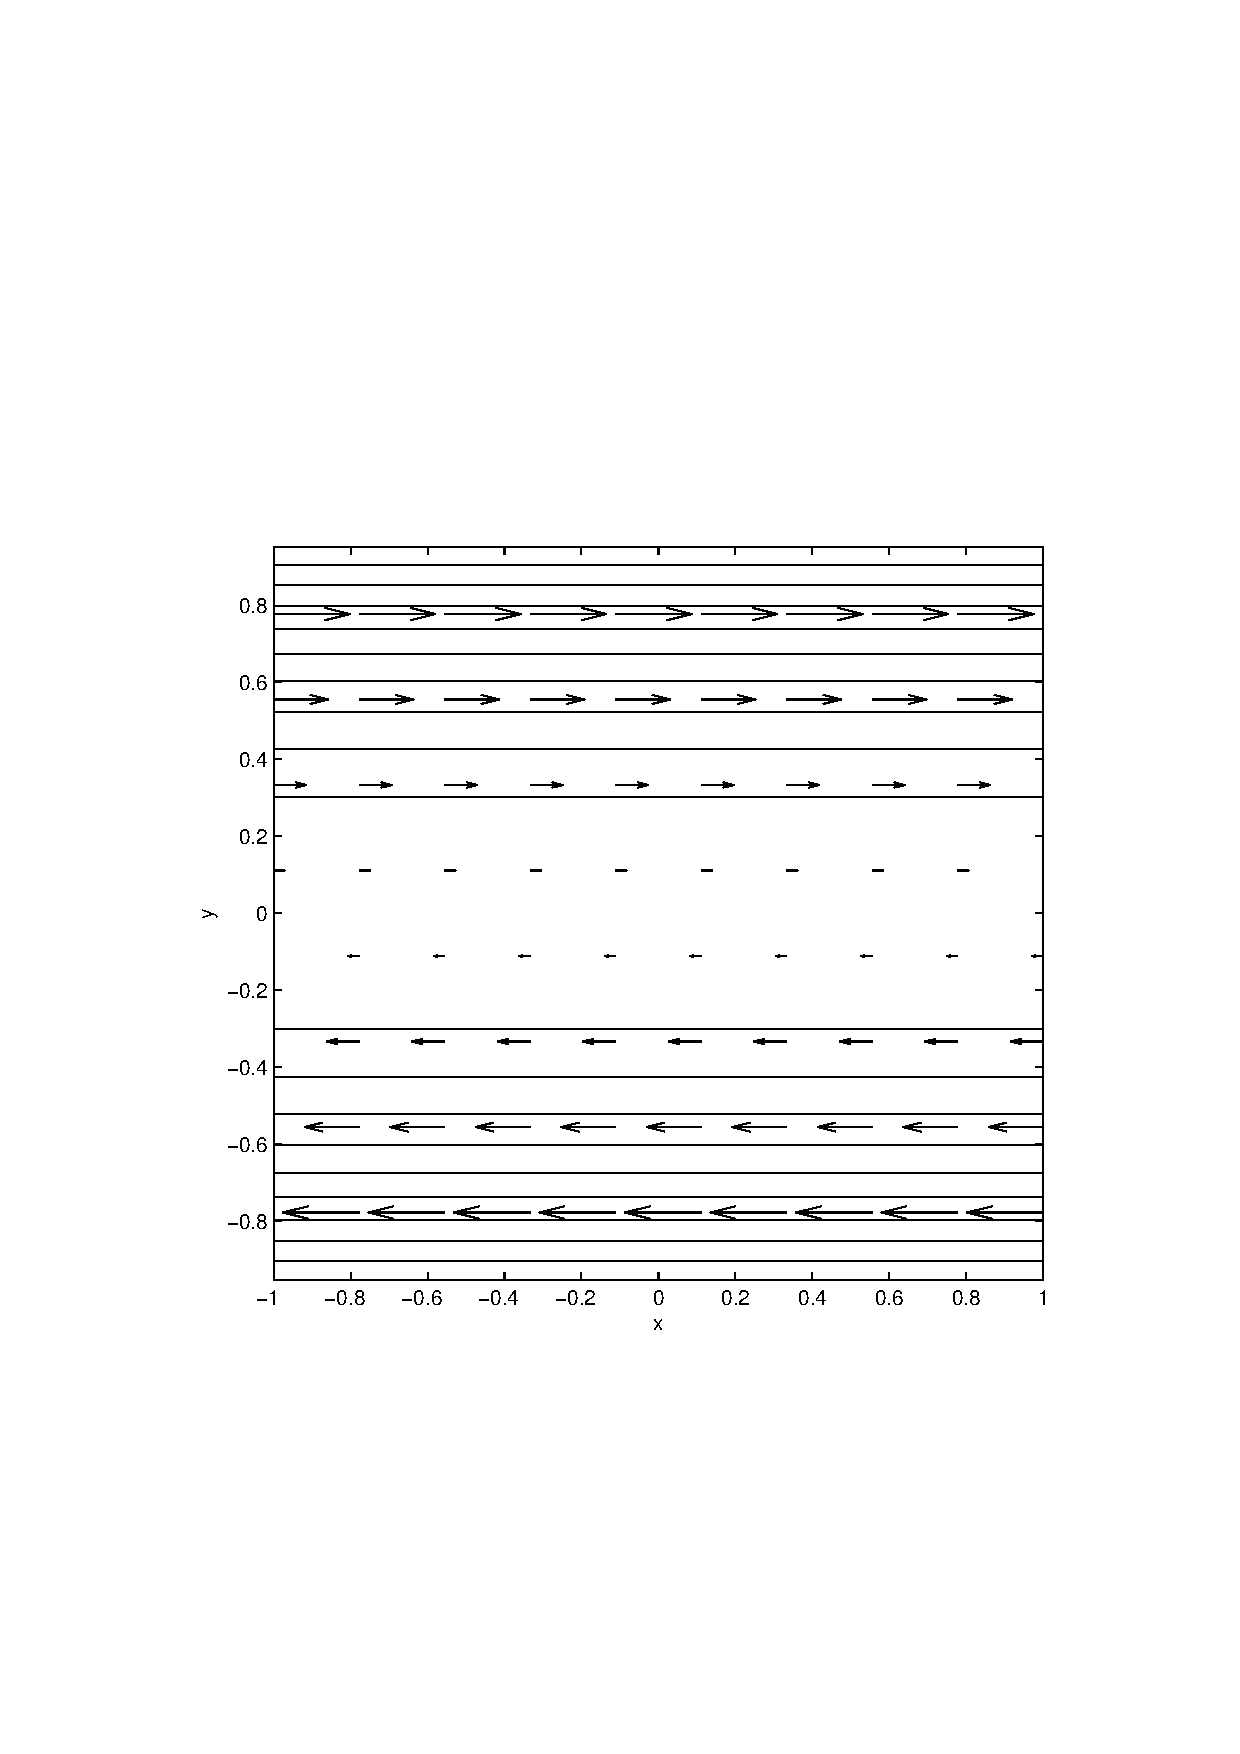
\includegraphics[height = 25mm]{streamlines.png}}{./Figures/trajectory.avi}
		}
	\end{picture}
\end{center}

\medskip

La visualisation expérimentale des lignes de courant s'effectue par la prise d'une photo 
à temps de pose court de l'écoulement ensemencé de particules réfléchissantes.
Les lignes de courant peuvent alors se déduire des courts segments de traînée lumineuse
laissée par les particules sur le cliché.

\medskip

{\bf Définitions : }

Une \textcolor{rouge}{surface de courant} est 
l'ensemble des lignes de courant s'appuyant sur un même contour fermé.

Un  \textcolor{rouge}{tube de courant} est le volume délimité par une surface de courant.


%\medskip
%{\bf Définitions : }
 
%On appelle {\em surface de courant} une surface générée par des lignes de courant contigües; 

%On appelle {\em tube de courant} un volume traversé par le fluide et délité par une (ou plusieurs) surface(s) de courant  

\vspace{0mm}

\end{frame}

%--------------------------------------------------------------------------------------------------
\subsubsection{Lignes d'émission}
%--------------------------------------------------------------------------------------------------
\begin{frame}{Lignes d'émission}
%--------------------------------------------------------------------------------------------------

\small

\mybaselineskip{1.2}{
	Une \textcolor{rouge}{ligne d'émission} 
	correspond à l'ensemble des positions occupées \textcolor{rouge}{à un instant donné $t$} \\
	par toutes les particules fluides qui sont passées auparavant 
	(à un instant antérieur $\tau < t	$) \\ 
	au même point géométrique $\myvec{X}_0$~:
}

\begin{equation*}
  \color{vert}
  \mathcal{E}(t) = \{ \myvec{X}(t, \myvec{X}_0) 
  \; / \; \exists \tau \in [0, t], \myvec{X}(\tau, \myvec{X}_0) = \myvec{X}_0 \}
\end{equation*}

\pause

\mybaselineskip{1.2}{
	La visualisation expérimentale d'une ligne d'émission s'effectue par la prise d'une photo
	\\ à l'instant $t$ d'un filet de colorant émis en continu 
	dans le fluide au point $\myvec{X}_0$.

\pause

	\medskip
	A titre d'exemple le panache de fumée d'une cigarette correspond à la ligne d'émission
	\\ provenant du bout incandescent.
}

\medskip

\begin{center}
	\begin{picture}(115, 28)
		\put(5, 0){\includegraphics[height = 30mm]{cigarette.jpg}} \pause
		\put(50, 0){\includegraphics[height = 30mm]{Manneken_pis.jpg}}
	\end{picture}
\end{center}

\vspace{0mm}

\end{frame}

%--------------------------------------------------------------------------------------------------
%\subsubsection{Exemple}
%--------------------------------------------------------------------------------------------------
\begin{frame}{Exemple}
%--------------------------------------------------------------------------------------------------

\small

  \vspace{3mm}

  \textbf{Ecoulement instationnaire derrière un cylindre}
    
  \begin{center}
    \begin{picture}(105, 35)(0, 0)
      \put( 0, 0){\includegraphics[width=50mm]{Fermigier1.png}}
      \put(55, 0){\includegraphics[width=50mm]{Fermigier2.png}}
      \put( 1, 1){(a)}
      \put(56, 1){(b)}
    \end{picture}
    
    \medskip
    \slshape \color{gris}(Le fluide va de gauche à droite
    et le cylindre se trouve à gauche juste en dehors de l'image)
  \end{center}
    
    \vspace{5mm}
    
    (a) Visualisation des lignes d'émission et du déplacement 
    des particules pendant le temps de pose.
    
    \smallskip
    
    (b) Reconstruction de quelques lignes de courant.
    
    \vspace{10mm}
    
    \hfill
    D'après le cours \textsl{Hydrodynamique Physique} de Marc Fermigier (ESPCI, 2002).

\vspace{10mm}

\end{frame}
%--------------------------------------------------------------------------------------------------
%\subsubsection{Propriété}
%--------------------------------------------------------------------------------------------------
\begin{frame}{Propriété}
%--------------------------------------------------------------------------------------------------

\small
\textcolor{vert}{\sl Exercice (MMC) :}

\medskip

\hspace*{10mm}
\begin{minipage}{100mm}
pour un écoulement stationnaire, on montre que ces trois familles de courbes \\
(trajectoires, lignes de courant et lignes d'émission) sont confondues.
\end{minipage}

\vspace{50mm}

\end{frame}

%==================================================================================================
\subsection{Fonction de courant}
%==================================================================================================
%--------------------------------------------------------------------------------------------------
\begin{frame}{Fonction de courant (écoulement 2D incompressible)}
%-------------------------------------------------------------------------------------------------- 

Considérons un écoulement bidimensionnel de la forme $\vec{u} = u_x \vec{e}_x +   u_y \vec{e}_y$.

\smallskip

{\bf Théorème } : 

Si $div(\vec u) = 0$, alors il existe une fonction $\psi(x,y)$ telle que 

$$
u_x = \frac{\partial \psi}{\partial y}  \, , \qquad u_y =  - \frac{\partial \psi}{\partial y} 
$$

\pause \medskip
{\bf Propriétés :}
\begin{itemize}
\item $\psi$ est constante le long des lignes de courant. {\color{vert} [Démo] }
\item Le flux volumique a travers un {\em tube de courant} bordé par deux lignes de courant d'équation $\psi = \psi_1$ et $\psi = \psi_2$
(et traversé par une surface transverse $\cal S$ vaut :
$$ \int_{\cal S}  \vec{u} \cdot  \vec {n} \, dS = \left| \psi_2 - \psi_1 \right| $$
\item[] NB : $[\psi] = m^2 s^{-1}$, l'expression précédente définit donc un flux volumique {\em par unité de largeur dans la direction transverse}.

\item On peut aussi écrire ${\vec u } = rot ( \psi \vec{e}_z)$.
\item $\vec{\omega} = rot ( \vec{u}) = - \Delta \psi \vec{e}_z$.


\item Si l'écoulement est décrit en {\em coordonnées polaires } par $\vec{u} = u_r \vec{e}_r +   u_\theta \vec{e}_\theta$ alors on peut utiliser $\psi(r,\theta)$:
$$
u_r = \frac{1}{r} \frac{\partial \psi}{\partial \theta}  \, , \qquad u_\theta =  - \frac{\partial \psi}{\partial r} 
$$



\end{itemize}
\end{frame}


%--------------------------------------------------------------------------------------------------
\begin{frame}{Fonction de Stokes (écoulement incompressible à symétrie de révolution)}
%-------------------------------------------------------------------------------------------------- 

Considérons un écoulement a {\em symétrie de révolution} de la forme $\vec{u} = u_r \vec{e}_r +   u_z \vec{e}_z$.

\smallskip

{\bf Théorème } : 

Si $div(\vec u) = 0$, alors il existe une fonction $\Psi(r,z)$ telle que 

$$
u_r = - \frac{1}{r}\frac{\partial \Psi}{\partial z}  \, , \qquad u_z =  \frac{1}{r} \frac{\partial \Psi}{\partial r} 
$$

\pause \medskip
{\bf Propriétés :}
\begin{itemize}
\item $\Psi$ est constante le long des surfaces de courant. {\color{vert} [Démo] }
\item Le flux volumique a travers un {\em tube de courant} bordé par deux surfaces de courant d'équation $\Psi = \Psi_1$ et $\Psi = \Psi_2$
(et traversé par une surface transverse $\cal S$) vaut :
$$ \int_{\cal S}  \vec{u} \cdot  \vec {n} \, dS = \left| \Psi_2 - \Psi_1 \right| $$
\item[] NB : $[\Psi] = m^3 s^{-1}$, l'expression précédente définit donc bien un flux volumique.

\item Si l'écoulement est décrit en {\em coordonnées sphériques } par $\vec{u} = u_R \vec{e}_R +   u_\Theta \vec{e}_\Theta$, alors on peut travailler a partir de la fonction $\Psi(R,\Theta)$ :
\begin{equation}
% \vec{u} = \rot ( \Psi(x,y)/r  \vec{e_z}), 
%\quad \mbox{ c.a.d :} \quad \quad 
%\left\{
%\begin{array}{ccc}
\displaystyle u_R &=& \displaystyle - \frac{1}{R^2 \sin \Theta }\frac{\partial \Psi}{\partial \Theta}, \qquad 
\displaystyle u_\Theta &=& \displaystyle  \frac{1}{R \sin \Theta}\frac{\partial \Psi}{\partial R}.
%\end{array}
%\right.
\end{equation}



\end{itemize}
\end{frame}

































\comment{
%--------------------------------------------------------------------------------------------------
\begin{frame}{Principes de conservation et formulation eulérienne}
%--------------------------------------------------------------------------------------------------

\small

\textbf{"Petit" inconvénient de la description eulérienne :} \medskip

les principes de conservation de la physique et les 
bilans fondamentaux de la Mécanique des Milieux Continus en particulier
trouvent leur formulation naturelle dans le cas d'un \textcolor{rouge}{système matériel donné} et en mouvement. 

\medskip

Un tel système est par définition constitué d'un ensemble donné de particules fluides et il faut donc écrire le bilan de grandeurs physiques \textbf{en suivant ces particules fluides dans leur mouvement}.

\pause

\medskip

Il faut ainsi être capable d'exprimer les dérivées temporelles des grandeurs pour chaque particule en fonction du champ eulérien et donc exprimer la variation temporelle de la vitesse (accélération) ou de toute autre grandeurs physique (masse volumique, température) 
\textbf{\textcolor{rouge}{en suivant la matière (une seule particule fluide ou un ensemble de particules fluides) dans son mouvement}}.

\vspace{5mm} \pause
 
\color{bleu}
 
\textbf{Objectif : } \medskip

\mybaselineskip{1.2}{
Connaissant le champ eulérien $f(\myvec{x}, t)$ d'une grandeur physique donnée en tout point géométrique $\myvec{x}$ et à chaque instant $t$, comment remonter à la 
\textbf{variation temporelle} de cette grandeur physique attachée à la particule fluide 
$F(t; \myvec{X}_0)$ lorsqu'on la \textbf{suit dans son mouvement} ?
}

\pause
\bigskip

\begin{center}
\color{rouge} 
\bf \begin{picture}(5, 0)\put(0, -0.7){\Large \ding{223}}\end{picture}
comment calculer $\dot{F}(t; \myvec{X}_0)$ connaissant $f(\myvec{x}, t)$ ?
\end{center}

\vspace{5mm}

\end{frame}


%--------------------------------------------------------------------------------------------------
\begin{frame}{Principes de conservation et formulation eulérienne}
%--------------------------------------------------------------------------------------------------

\small

\textbf{Exemples :} \medskip 

\mybaselineskip{1.2}{
on souhaite ainsi remonter à : 

\begin{itemize}
\item
la variation au cours du temps de la température $T(t; \myvec{X}_0)$ 
de la particule $\myvec{X}_0$ connaissant le champ eulérien de température 
$T(\myvec{x}, t)$ en tout point de l'espace à chaque instant : comment
calculer $\dot{T}(t; \myvec{X}_0)$ en fonction de $h(\myvec{x}, t)$ ?
\item
l'accélération de la particule fluide, c'est-à-dire
la variation au cours du temps de la vitesse des particules fluides, 
$\dot{\myvec{X}}(t; \myvec{X}_0)$ ?
\item
la variation au cours du temps de l'énergie cinétique totale d'un ensemble donné de particules fluides 
$$\displaystyle E_k(t) = \int_{\mathcal{D}(t)}\dfrac{1}{2} \myvec{u}^2(\myvec{x}, t)\, \rho(\myvec{x}, t) \; dV$$
pour calculer $\dot{E}_k = dE_k/dt$ connaissant les champs eulériens de masse volumique $\rho(\myvec{x}, t)$
et de vitesse $\myvec{u}(\myvec{x}, t)$.
\end{itemize}
}
\medskip

\begin{center}
$\rightarrow$ concept de \textcolor{rouge}{dérivée particulaire}
\end{center}

\vspace{10mm}

\end{frame}
}


\comment{
%--------------------------{------------------------------------------------------------------------
%\subsubsection{Quantité intégrale}
%--------------------------------------------------------------------------------------------------
\begin{frame}{Dérivée matérielle d'une quantité intégrale}
%--------------------------------------------------------------------------------------------------

\small
Soit la quantité extensive $\mathcal{F}$ associée à la quantité intensive représentée 
par le champ eulérien $f(\myvec{x}, t)$ (par exemple la masse et la masse volumique).

\medskip
\pause 

Dans un formalisme Eulérien on considère naturellement des intégrales sur un \textcolor{vert}{volume de contrôle} fixe $\Omega$ :

$$
 \mathcal{F}_\Omega = \int_\Omega f(\myvec{x}, t)\, dV 
$$

\medskip
\pause

En revanche les lois de la physique s'écrivent plus naturellement pour des quantités intégrées sur un \textcolor{vert}{volume matériel} ${\cal D}(t)$ se déplaçant avec le fluide :
 
$$
 \mathcal{F}_{{\cal D}(t)} = \int_{{\cal D}(t)} f(\myvec{x}, t)\, dV 
$$

\medskip 
\pause

Comment exprimer les dérivées temporelles dans un cas et dans l'autre ?


\medskip 
\pause

On montre que :

$$
\frac{d }{dt} \mathcal{F}_\Omega
=  \int_\Omega \dpdt{} f \, dV
$$

\medskip 
\pause

$$
\frac{d }{dt} \mathcal{F}_{{\cal D}(t)}
=  \frac{d }{dt} \mathcal{F}_\Omega +  \oint_{\partial\Omega} f\myvec{u}\cdot\myvec{n}\, dS
$$



%Pour tout \textcolor{vert}{volume de contrôle} $\Omega$ fixe en espace, on suppose connue à chaque instant la quantité  
%\[
%	\mathcal{F}(t) = \int_\Omega f(\myvec{x}, t)\, dV
%\]

%On souhaite connaître la variation au cours du temps de la quantité extensive $\mathcal{F}$ lorsque l'on suit dans son mouvement la matière contenue à l'instant $t$ dans $\Omega$.
%
%\medskip
%\pause
%Soit alors $\mathcal{D}(t)$ le \textcolor{vert}{volume matériel} de fluide coïncidant à l'instant $t$ avec le volume de contrôle $\Omega$.
%
%A l'instant $t$ :
%\[
%	\mathcal{F}(t) = \int_{\mathcal{D}(t) = \Omega} f(\myvec{x}, t)\, dV
%\]
%
%A l'instant $t+dt$, ce volume de matière s'est déplacé en $\mathcal{D}(t+dt) = \Omega'$ :
%\[
%	\mathcal{F}(t+dt) = \int_{\mathcal{D}(t+dt) = \Omega'} f(\myvec{x}, t+dt)\, dV
%\]
%
%\medskip
%\pause
%
%On montre que \quad
%$ \color{rouge}
%  \displaystyle
%	\dot{\mathcal{F}}(t) = \lim_{dt\rightarrow 0} \frac{\mathcal{F}(t+dt) - \mathcal{F}(t)}{dt}
%	=   \dpdt{} \int_\Omega f\, dV + \oint_{\partial\Omega} f\myvec{u}\cdot\myvec{n}\, dS
%$
%
%\medskip
%où $\partial \Omega$ désigne la frontière du volume de contrôle $\Omega$, 
%de normale sortante $\myvec{n}$.
%
%\bigskip
%
%
\textcolor{vert}{\sl Exercice (MMC) :} démontrer cette relation, de manière formelle ou géométrique.

\vspace{0mm}

\end{frame}

%--------------------------------------------------------------------------------------------------
\begin{frame}{Théorème du transport de Reynolds}
%--------------------------------------------------------------------------------------------------

\small

On en déduit l'expression de la dérivée particulaire de la quantité intégrale 
\[
	\mathcal{F}(t) = \int_{{\cal D}(t)} f(\myvec{x}, t)\, dV,
\]
correspondant au taux de variation de $\mathcal{F}$ en suivant la matière dans son mouvement :

\[
	\color{rouge}
	\ddt{\mathcal{F}} 
	= 
	\dpdt{} \int_\Omega f\, dV + \oint_{\partial\Omega} f\myvec{u}\cdot\myvec{n}\, dS
\]

$\longrightarrow$ $\dpdt{} \int_\Omega f\, dV$ correspond à la variation temporelle de la quantité $f$
dans le volume $\Omega$.

\smallskip

$\longrightarrow$ $\displaystyle \oint_{\partial\Omega} f\myvec{u}\cdot\myvec{n}\, dS$ correspond au \textcolor{rouge}{flux}
de la quantité $f$ à travers la frontière de $\Omega$.

\pause
\bigskip

Autre écriture, par application du \textcolor{vert}{théorème de la divergence} :

\medskip
\pause

[Démonstration\ldots] \qquad $\longrightarrow$ \qquad
$ \displaystyle \color{rouge}	
\ddt{\mathcal{F}} = 
\int_\Omega \left [{\color{rouge}\ddt{f}} + f\divergence (\myvec{u})\right ] \, dV
$

%\vspace{10mm}
\medskip
\pause 

Application : posons $f=1$. On obtient :
\smallskip
$	
\ddt{\mathcal{V}} = 
\int_\Omega  \divergence (\myvec{u})  \, dV
$

\smallskip
La divergence du champ de vitesse s'interprète donc comme le taux de dilatation volumique de l'écoulement.

Si $\divergence (\myvec{u}) = 0$ on parle d'écoulement isovolume.
On parle aussi d' "écoulement incompressible" ; mais c'est un abus de language ! 

(la compressibilité est une propriété du fluide, pas de l'écoulement). 

Un gaz (compressible) tout comme un liquide (souvent modélisé comme incompressible) peuvent s'écouler de manière iso-volume...



\end{frame}
}



